\documentclass[a4paper,12pt]{article}

% --- Подключение пакетов ---
\usepackage[T2A]{fontenc}
\usepackage[utf8]{inputenc}
\usepackage[russian]{babel}

\usepackage{amsmath}
\usepackage{amssymb}
\usepackage{amsfonts} % Мат. символы

\usepackage{graphicx} % Для вставки картинок
\usepackage{geometry} % Поля страницы
\usepackage{listings} % Для вставки кода
\usepackage{xcolor}   % Цвета для кода
\usepackage{hyperref} % Гиперссылки
\usepackage{float}    % Плавающие объекты

% --- Настройка полей ---
\geometry{left=2cm, right=1.5cm, top=2cm, bottom=2cm}

% --- Авторская настройка для адекватной вставки кода с использованием кириллицы ---
\lstdefinestyle{mypython}{
    language=Python,
    basicstyle=\ttfamily\scriptsize,
    keywordstyle=\color{blue}\bfseries,
    stringstyle=\color{red},
    commentstyle=\color{green!60!black},
    numbers=left,
    numberstyle=\tiny\color{gray},
    stepnumber=1,
    numbersep=8pt,
    showspaces=false,
    showstringspaces=false,
    tabsize=4,
    frame=single,
    rulecolor=\color{black},
    breaklines=true,
    breakatwhitespace=false,
    captionpos=b,
    xleftmargin=15pt,
    xrightmargin=5pt,
    framexleftmargin=12pt,
    backgroundcolor=\color{gray!5},
    literate=%
        {а}{{\cyra}}1 {б}{{\cyrb}}1 {в}{{\cyrv}}1 {г}{{\cyrg}}1 {д}{{\cyrd}}1
        {е}{{\cyre}}1 {ё}{{\cyrie}}1 {ж}{{\cyrzh}}1 {з}{{\cyrz}}1 {и}{{\cyri}}1
        {й}{{\cyrishrt}}1 {к}{{\cyrk}}1 {л}{{\cyrl}}1 {м}{{\cyrm}}1 {н}{{\cyrn}}1
        {о}{{\cyro}}1 {п}{{\cyrp}}1 {р}{{\cyrr}}1 {с}{{\cyrs}}1 {т}{{\cyrt}}1
        {у}{{\cyru}}1 {ф}{{\cyrf}}1 {х}{{\cyrh}}1 {ц}{{\cyrc}}1 {ч}{{\cyrch}}1
        {ш}{{\cyrsh}}1 {щ}{{\cyrshch}}1 {ъ}{{\cyrhrdsn}}1 {ы}{{\cyrery}}1
        {ь}{{\cyrsftsn}}1 {э}{{\cyrerev}}1 {ю}{{\cyryu}}1 {я}{{\cyrya}}1
        {А}{{\CYRA}}1 {Б}{{\CYRB}}1 {В}{{\CYRV}}1 {Г}{{\CYRG}}1 {Д}{{\CYRD}}1
        {Е}{{\CYRE}}1 {Ё}{{\CYRIE}}1 {Ж}{{\CYRZH}}1 {З}{{\CYRZ}}1 {И}{{\CYRI}}1
        {Й}{{\CYRISHRT}}1 {К}{{\CYRK}}1 {Л}{{\CYRL}}1 {М}{{\CYRM}}1 {Н}{{\CYRN}}1
        {О}{{\CYRO}}1 {П}{{\CYRP}}1 {Р}{{\CYRR}}1 {С}{{\CYRS}}1 {Т}{{\CYRT}}1
        {У}{{\CYRU}}1 {Ф}{{\CYRF}}1 {Х}{{\CYRH}}1 {Ц}{{\CYRC}}1 {Ч}{{\CYRCH}}1
        {Ш}{{\CYRSH}}1 {Щ}{{\CYRSHCH}}1 {Ъ}{{\CYRHRDSN}}1 {Ы}{{\CYRERY}}1
        {Ь}{{\CYRSFTSN}}1 {Э}{{\CYREREV}}1 {Ю}{{\CYRYU}}1 {Я}{{\CYRYA}}1
}
\lstset{style=mypython}

\begin{document}

% ===========================================================================
% 1. ТИТУЛЬНЫЙ ЛИСТ
% ===========================================================================
\begin{titlepage}
    \centering
    % Шапка
    {\fontsize{11}{13}\selectfont \textbf{Министерство науки и высшего образования Российской Федерации}} \\
    {\fontsize{7}{10}\selectfont ФЕДЕРАЛЬНОЕ ГОСУДАРСТВЕННОЕ АВТОНОМНОЕ ОБРАЗОВАТЕЛЬНОЕ УЧРЕЖДЕНИЕ ВЫСШЕГО ОБРАЗОВАНИЯ} \\
    \vspace{0.2cm} 
    {\fontsize{14}{17}\selectfont \textbf{«НАЦИОНАЛЬНЫЙ ИССЛЕДОВАТЕЛЬСКИЙ УНИВЕРСИТЕТ ИТМО»}}
    
    \vspace{1cm} 
    
    % Информация о группе
    {\fontsize{12}{14}\selectfont \textbf{Группа P3211}}
    
    \vspace{1cm}
    
    % Информация о дисциплине
    {\fontsize{12}{14}\selectfont \textbf{Дисциплина: Вычислительная математика}}
    
    \vspace*{\fill}
    
    % Заголовок работы
    {\fontsize{18}{22}\selectfont \textbf{ЛАБОРАТОРНАЯ РАБОТА №2}} \\
    \vspace{0.5cm}
    {\fontsize{14}{17}\selectfont \textbf{по теме: «Численное решение нелинейных уравнений и систем»}}
    
    \vspace{2cm}
    
    {\fontsize{12}{14}\selectfont \textbf{Вариант 11}}
    
    \vspace{2cm}
    
    % Блок выполнил/проверил
    \begin{flushright}
        \fontsize{12}{14}\selectfont
        Выполнил: \\
        Михайлов Петр Сергеевич \\
        \vspace{1em}
        Преподаватель: \\
        Малышева Татьяна Алексеевна
    \end{flushright}
    
    \vfill
    
    % Подвал
    {\fontsize{12}{14}\selectfont
    Санкт-Петербург, 2026
    }
\end{titlepage}

\setcounter{page}{2}

\newpage

% ===========================================================================
% 2. Оглавление
% ===========================================================================
\tableofcontents

\newpage

% ===========================================================================
% 3. Цель работы
% ===========================================================================
\section{Цель работы}
Изучить численные методы решения нелинейных уравнений и их систем, найти корни заданного нелинейного уравнения и системы нелинейных уравнений, выполнить программную реализацию методов.

% ===========================================================================
% 4. Порядок выполнения работы
% ===========================================================================
\section{Порядок выполнения работы}
\begin{enumerate}
    \item Отделить корни заданного нелинейного уравнения графически или аналитически.
    \item Определить интервалы изоляции корней.
    \item Уточнить корни нелинейного уравнения с точностью $\epsilon=10^{-2}$ выбранными методами.
    \item Отделить корни заданной системы нелинейных уравнений графически.
    \item Решить систему нелинейных уравнений заданным методом с точностью до 0,01.
    \item Выполнить программную реализацию численных методов.
    \item Оформить отчет по результатам вычислительной и программной реализации.
\end{enumerate}

% ===========================================================================
% 5. Рабочие формулы используемых методов
% ===========================================================================
\section{Рабочие формулы используемых методов}
В рамках лабораторной работы применялись следующие численные методы:
\begin{itemize}
    \item \textbf{Метод половинного деления (дихотомии):}
    \begin{equation}
        x_i = \frac{a_i + b_i}{2}
    \end{equation}
    Условие выбора нового интервала: если $f(a_i) \cdot f(x_i) < 0$, то $b_{i+1} = x_i$, иначе $a_{i+1} = x_i$.

    \item \textbf{Метод секущих:}
    \begin{equation}
        x_{k+1} = x_k - \frac{x_k - x_{k-1}}{f(x_k) - f(x_{k-1})} f(x_k)
    \end{equation}

    \item \textbf{Метод простой итерации (для нелинейного уравнения):}
    Уравнение приводится к эквивалентному виду $x = \varphi(x)$, где $\varphi(x) = x + \lambda f(x)$. Значение $\lambda$ выбирается исходя из условия сходимости $\max |\varphi'(x)| < 1$. Итерационный процесс:
    \begin{equation}
        x_{k+1} = \varphi(x_k)
    \end{equation}

    \item \textbf{Метод Ньютона (для систем нелинейных уравнений):}
    Для системы $\begin{cases} f(x, y) = 0 \\ g(x, y) = 0 \end{cases}$ строится матрица Якоби:
    \begin{equation}
        J(x, y) = \begin{pmatrix} \frac{\partial f}{\partial x} & \frac{\partial f}{\partial y} \\ \frac{\partial g}{\partial x} & \frac{\partial g}{\partial y} \end{pmatrix}
    \end{equation}
    На каждом шаге решается СЛАУ относительно приращений $\Delta x, \Delta y$:
    \begin{equation}
        J(x_k, y_k) \begin{pmatrix} \Delta x \\ \Delta y \end{pmatrix} = -\begin{pmatrix} f(x_k, y_k) \\ g(x_k, y_k) \end{pmatrix}
    \end{equation}
    Новые приближения: $x_{k+1} = x_k + \Delta x$, $y_{k+1} = y_k + \Delta y$.
\end{itemize}

% ===========================================================================
% 6. Графики функций на исследуемом интервале
% ===========================================================================
\newpage
\section{Графики функций на исследуемом интервале}

\subsection{Локализация корней нелинейного уравнения}
Задано нелинейное уравнение (Вариант 11):
\begin{equation}
    f(x) = 4,45x^3 + 7,81x^2 - 9,62x - 8,17 = 0
\end{equation}

\begin{figure}[H]
    \centering
    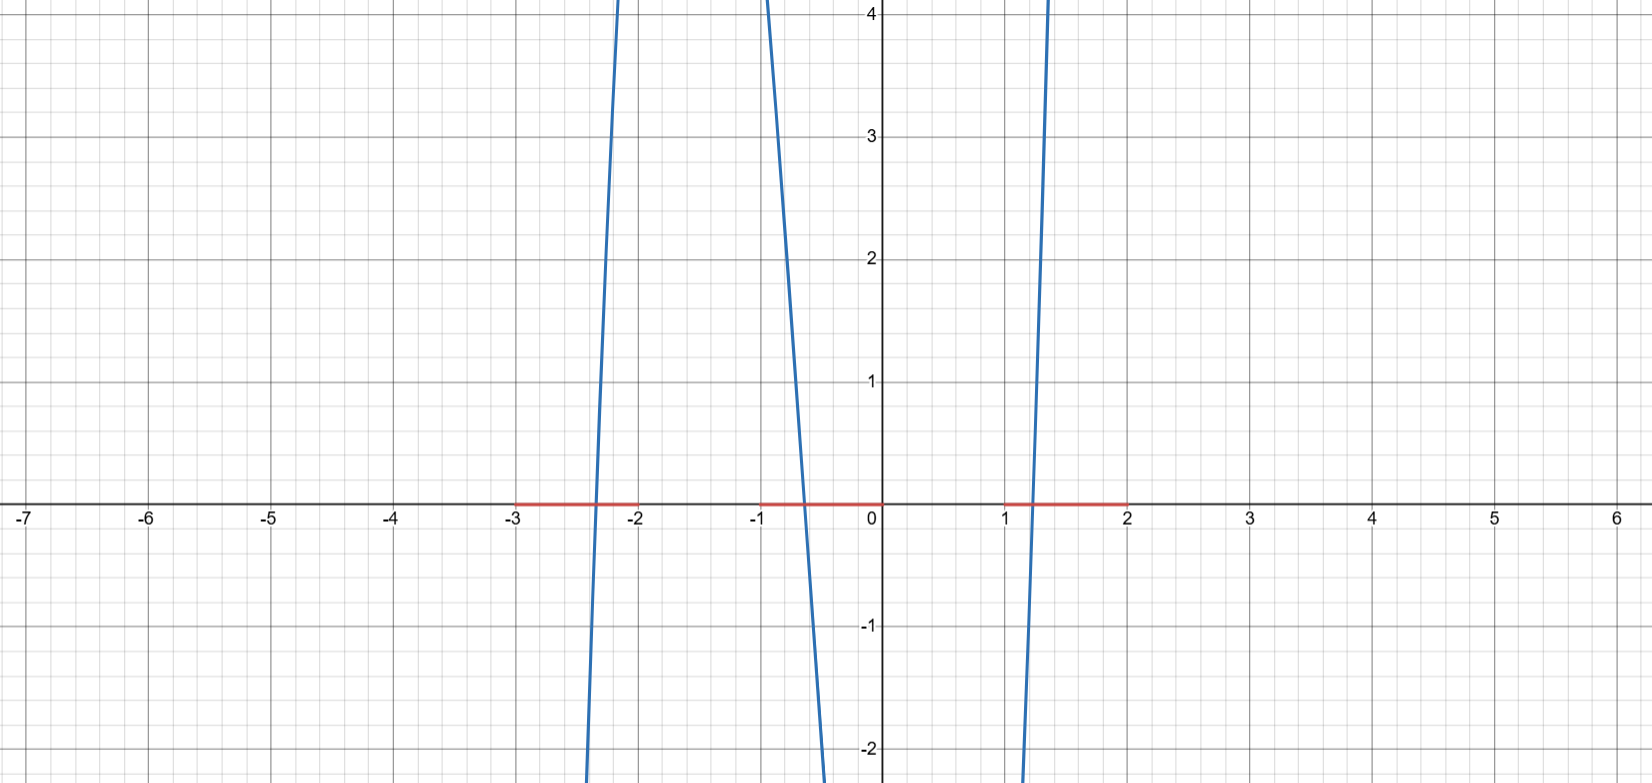
\includegraphics[width=0.8\textwidth]{graph_equation_1.1.png}
    \caption{График функции $f(x) = 4,45x^3 + 7,81x^2 - 9,62x - 8,17$}
\end{figure}

Найдем экстремумы функции аналитически, приравняв производную к нулю:
\begin{equation}
    f'(x) = 13,35x^2 + 15,62x - 9,62 = 0
\end{equation}
Корни производной (точки локального экстремума): $x \approx -1,616$ (максимум, $f(x) \approx 8,99$) и $x \approx 0,446$ (минимум, $f(x) \approx -10,51$). Поскольку значения функции в точках экстремумов имеют разные знаки, уравнение имеет ровно 3 действительных корня.

Из графика и аналитического расчета определяем интервалы изоляции:
\begin{itemize}
    \item Крайний левый корень: $x \in [-3; -2]$
    \item Центральный корень: $x \in [-1; 0]$
    \item Крайний правый корень: $x \in [1; 2]$
\end{itemize}

% ===========================================================================
% 7. Заполненные таблицы вычислительной части 1
% ===========================================================================
\newpage
\section{Заполненные таблицы вычислительной части 1}
Точность вычислений: $\epsilon = 10^{-2}$.

\subsection{Уточнение крайнего правого корня методом половинного деления}

Идея метода заключается в том, что начальный интервал изоляции корня делится пополам, в результате чего получается начальное приближение к корню $x_0 = \frac{a_0 + b_0}{2}$. Затем вычисляется значение функции $f(x_0)$. В качестве нового интервала выбирается та половина отрезка ($[a_0, x_0]$ или $[b_0, x_0]$), на концах которого функция имеет разные знаки. Другая половина отрезка, на которой функция не меняет знак, отбрасывается. Рабочая формула метода: $x_i = \frac{a_i + b_i}{2}$. В качестве одного из критериев окончания итерационного процесса можно использовать $|a_n - b_n| \le \epsilon$.

Для интервала $[1; 2]$ функция меняет знак: $f(1) = -5,530$, $f(2) = 39,430$.

\begin{table}[H]
\centering
\begin{tabular}{|c|c|c|c|c|c|c|c|}
\hline
№ шага & $a$ & $b$ & $x$ & $f(a)$ & $f(b)$ & $f(x)$ & $|a-b|$ \\ \hline
1 & 1,000 & 2,000 & 1,500 & -5,530 & 39,430 & 9,991 & 1,000 \\ \hline
2 & 1,000 & 1,500 & 1,250 & -5,530 & 9,991 & 0,699 & 0,500 \\ \hline
3 & 1,000 & 1,250 & 1,125 & -5,530 & 0,699 & -2,772 & 0,250 \\ \hline
4 & 1,125 & 1,250 & 1,188 & -2,772 & 0,699 & -1,129 & 0,125 \\ \hline
5 & 1,188 & 1,250 & 1,219 & -1,129 & 0,699 & -0,237 & 0,063 \\ \hline
6 & 1,219 & 1,250 & 1,234 & -0,237 & 0,699 & 0,226 & 0,031 \\ \hline
7 & 1,219 & 1,234 & 1,227 & -0,237 & 0,226 & -0,007 & 0,015 \\ \hline
\end{tabular}
\caption{Уточнение корня методом половинного деления}
\end{table}
\textbf{Ответ:} Крайний правый корень $x \approx 1,227$.

\subsection{Уточнение крайнего левого корня методом секущих}

Данный метод упрощает метод Ньютона, заменяя производную $f'(x)$ разностным приближением: $f'(x_i) \approx \frac{f(x_i) - f(x_{i-1})}{x_i - x_{i-1}}$. Метод секущих является двухшаговым, то есть новое приближение $x_{i+1}$ определяется двумя предыдущими итерациями $x_i$ и $x_{i-1}$. Рабочая формула метода: $x_{i+1} = x_i - \frac{x_i - x_{i-1}}{f(x_i) - f(x_{i-1})} f(x_i)$. Критерием окончания процесса выступает $ |x_n - x_{n-1}| \le \epsilon $ или $ |f(x_n)| \le \epsilon $.

Для интервала $[-3; -2]$ заданы начальные приближения $x_0 = -3$ и $x_1 = -2,9$.

\begin{table}[H]
\centering
\begin{tabular}{|c|c|c|c|c|c|}
\hline
№ итерации & $x_{k-1}$ & $x_k$ & $x_{k+1}$ & $f(x_{k+1})$ & $|x_{k+1}-x_k|$ \\ \hline
1 & -3,000 & -2,900 & -2,518 & -5,472 & 0,382 \\ \hline
2 & -2,900 & -2,518 & -2,399 & -1,593 & 0,119 \\ \hline
3 & -2,518 & -2,399 & -2,351 & -0,199 & 0,048 \\ \hline
4 & -2,399 & -2,351 & -2,344 & -0,008 & 0,007 \\ \hline
\end{tabular}
\caption{Уточнение корня методом секущих}
\end{table}
\textbf{Ответ:} Крайний левый корень $x \approx -2,344$.

\subsection{Уточнение центрального корня методом простой итерации}

Суть метода состоит в том, что уравнение $f(x) = 0$ приводится к эквивалентному виду $x = \varphi(x)$ путем выражения $x$ из исходного уравнения. Если непосредственное преобразование не позволяет получить уравнение, удовлетворяющее условиям сходимости, применяется прием введения параметра $\lambda$, в результате чего $\varphi(x) = x + \lambda f(x)$. Зная начальное приближение $x_0$, очередные приближения вычисляются по рабочей формуле метода: $x_{i+1} = \varphi(x_i)$. Достаточное условие сходимости метода: $\max |\varphi'(x)| \le q < 1$. В качестве критерия окончания итерационного процесса можно ограничиться условием $|x_n - x_{n-1}| \le \epsilon$.

На интервале $[-1; 0]$ производная функции отрицательна. Выберем параметр $\lambda = 0,07$ для сведения уравнения к виду $x = \varphi(x) = x + 0,07 \cdot f(x)$.
Тогда $\varphi(x) = 0,3115x^3 + 0,5467x^2 + 0,3266x - 0,5719$.
На отрезке $\max |\varphi'(x)| \approx 0,3266 < 1$, достаточное условие сходимости выполняется. Выберем начальное приближение $x_0 = -0,5$.

\begin{table}[H]
\centering
\begin{tabular}{|c|c|c|c|c|}
\hline
№ итерации & $x_k$ & $x_{k+1}$ & $f(x_{k+1})$ & $|x_{k+1}-x_k|$ \\ \hline
1 & -0,500 & -0,637 & -0,019 & 0,137 \\ \hline
2 & -0,637 & -0,638 & -0,010 & 0,001 \\ \hline
3 & -0,638 & -0,639 & 0,005 & 0,001 \\ \hline
\end{tabular}
\caption{Уточнение корня уравнения методом простой итерации}
\end{table}
\textbf{Ответ:} Центральный корень $x \approx -0,639$.

% ===========================================================================
% 8. Решение системы нелинейных уравнений методом Ньютона
% ===========================================================================
\newpage
\section{Решение системы нелинейных уравнений}

Задана система нелинейных уравнений:
\begin{equation}
    \begin{cases}
        f_1(x, y) = \text{tg}(xy + 0,2) - x^2 = 0 \\
        f_2(x, y) = x^2 + 2y^2 - 1 = 0
    \end{cases}
\end{equation}

\subsection{Графическое отделение корней}
Для локализации корней построим графики функций. Второе уравнение — это эллипс с полуосями $a=1$ и $b \approx 0,707$. Первое уравнение — периодическая функция, напоминающая тангенсоиду.

\begin{figure}[H]
    \centering
    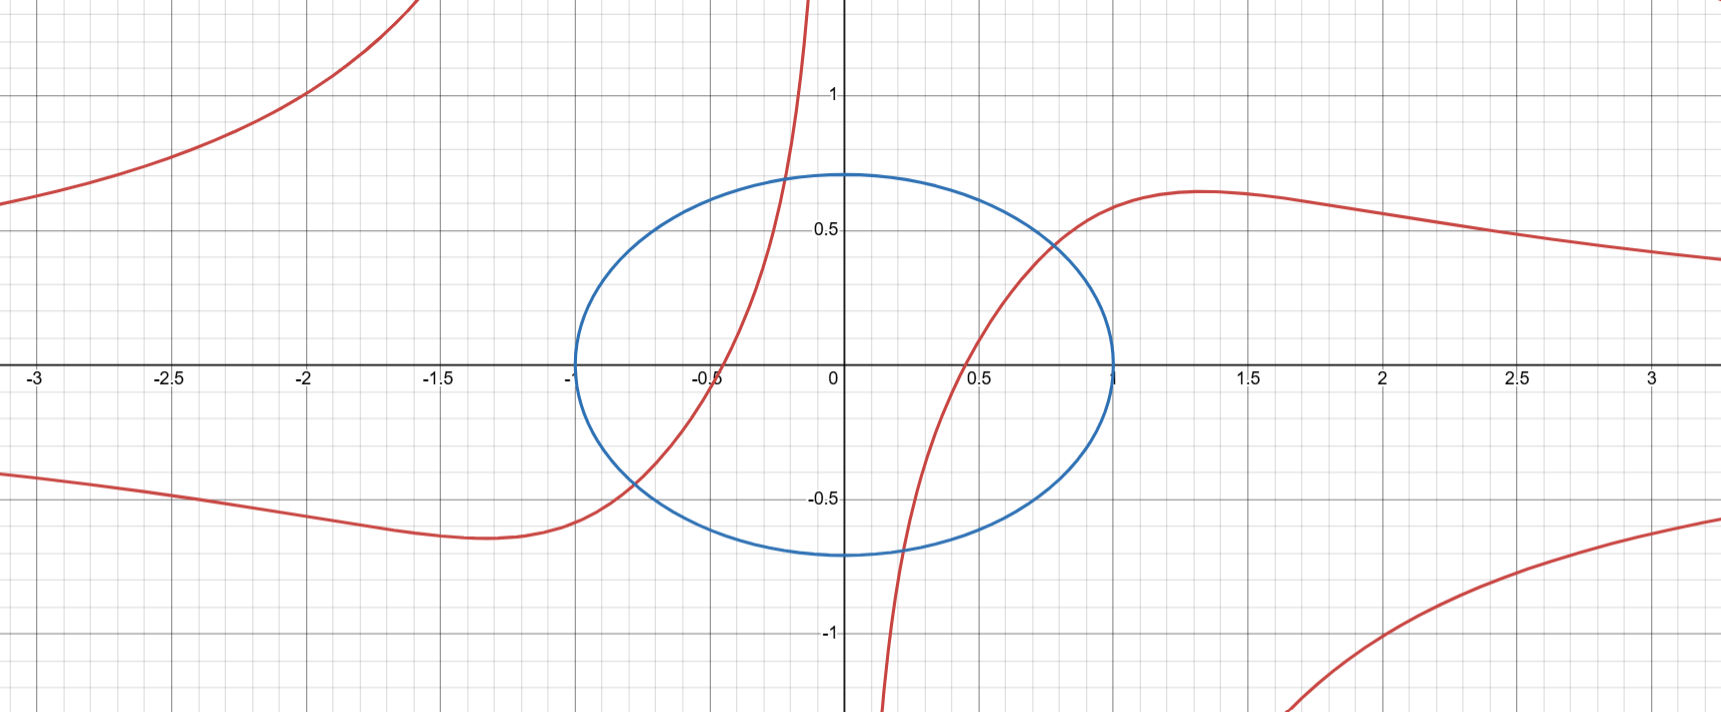
\includegraphics[width=0.7\textwidth]{graph_system_1.2.png}
    \caption{Графическое отделение корней системы}
\end{figure}

\textbf{Примечание:} Из графика видно, что система имеет 4 корня (по одному в каждой четверти). В данной работе мы будем уточнять только один корень, находящийся в первой четверти, так как алгоритм нахождения остальных корней идентичен и отличается только выбором начального приближения.

Выберем начальное приближение: $x_0 = 0,800$, $y_0 = 0,400$.

\subsection{Теоретические сведения}
Для уточнения корней используем метод Ньютона. Поправки $\Delta x$ и $\Delta y$ на каждой итерации находятся из СЛАУ:
\begin{equation}
\begin{pmatrix} 
\frac{\partial f_1}{\partial x} & \frac{\partial f_1}{\partial y} \\ 
\frac{\partial f_2}{\partial x} & \frac{\partial f_2}{\partial y} 
\end{pmatrix} 
\begin{pmatrix} \Delta x \\ \Delta y \end{pmatrix} = 
\begin{pmatrix} -f_1(x_k, y_k) \\ -f_2(x_k, y_k) \end{pmatrix}
\end{equation}

Частные производные:
\begin{itemize}
    \item $a_{11} = \frac{\partial f_1}{\partial x} = \frac{y}{\cos^2(xy+0,2)} - 2x$
    \item $a_{12} = \frac{\partial f_1}{\partial y} = \frac{x}{\cos^2(xy+0,2)}$
    \item $a_{21} = \frac{\partial f_2}{\partial x} = 2x$
    \item $a_{22} = \frac{\partial f_2}{\partial y} = 4y$
\end{itemize}

\subsection{Вычислительный процесс}

\subsubsection*{Итерация №1}
\textbf{1. Текущее приближение:} $x_0 = 0,800$; $y_0 = 0,400$. \\
\textbf{2. Значения функций:}
\begin{itemize}
    \item $f_1(0,8; 0,4) = \text{tg}(0,8 \cdot 0,4 + 0,2) - 0,8^2 = \text{tg}(0,52) - 0,64 \approx 0,573 - 0,64 = -0,067$
    \item $f_2(0,8; 0,4) = 0,8^2 + 2 \cdot 0,4^2 - 1 = 0,64 + 0,32 - 1 = -0,040$
\end{itemize}
\textbf{3. Значения элементов матрицы Якоби ($\cos^2(0,52) \approx 0,753$):}
\begin{itemize}
    \item $a_{11} = 0,4 / 0,753 - 1,6 \approx -1,069$
    \item $a_{12} = 0,8 / 0,753 \approx 1,062$
    \item $a_{21} = 2 \cdot 0,8 = 1,600$
    \item $a_{22} = 4 \cdot 0,4 = 1,600$
\end{itemize}
\textbf{4. Решение СЛАУ:}
\begin{equation*}
\begin{cases} -1,069 \Delta x + 1,062 \Delta y = 0,067 \\ 1,600 \Delta x + 1,600 \Delta y = 0,040 \end{cases} \implies
\begin{cases} \Delta x_0 \approx -0,019 \\ \Delta y_0 \approx 0,044 \end{cases}
\end{equation*}
\textbf{5. Новое приближение:} $x_1 = 0,781$; $y_1 = 0,444$. \\
\textbf{6. Погрешность:} $\delta = \max(|\Delta x|, |\Delta y|) = 0,044 > 0,01$. Продолжаем итерации.

\subsubsection*{Итерация №2}
\textbf{1. Текущее приближение:} $x_1 = 0,781$; $y_1 = 0,444$. \\
\textbf{2. Значения функций:}
\begin{itemize}
    \item $f_1(0,781; 0,444) = \text{tg}(0,547) - 0,610 \approx 0,609 - 0,610 = -0,001$
    \item $f_2(0,781; 0,444) = 0,610 + 0,394 - 1 = 0,004$
\end{itemize}
\textbf{3. Значения элементов матрицы Якоби ($\cos^2(0,547) \approx 0,729$):}
\begin{itemize}
    \item $a_{11} = 0,444 / 0,729 - 1,562 \approx -0,953$
    \item $a_{12} = 0,781 / 0,729 \approx 1,071$
    \item $a_{21} = 2 \cdot 0,781 = 1,562$
    \item $a_{22} = 4 \cdot 0,444 = 1,776$
\end{itemize}
\textbf{4. Решение СЛАУ:}
\begin{equation*}
\begin{cases} -0,953 \Delta x + 1,071 \Delta y = 0,001 \\ 1,562 \Delta x + 1,776 \Delta y = -0,004 \end{cases} \implies
\begin{cases} \Delta x_1 \approx -0,002 \\ \Delta y_1 \approx -0,001 \end{cases}
\end{equation*}
\textbf{5. Новое приближение:} $x_2 = 0,779$; $y_2 = 0,443$. \\
\textbf{6. Погрешность:} $\delta = \max(0,002; 0,001) = 0,002 < 0,01$. Условие точности выполнено.

\subsection{Результаты вычислений}
Сводная таблица уточнения корней:
\begin{table}[H]
\centering
\begin{tabular}{|c|c|c|c|c|c|c|c|}
\hline
$k$ & $x_k$ & $y_k$ & $f_1(x_k, y_k)$ & $f_2(x_k, y_k)$ & $\Delta x_k$ & $\Delta y_k$ & $\delta$ \\ \hline
0 & 0,800 & 0,400 & -0,067 & -0,040 & -0,019 & 0,044 & 0,044 \\ \hline
1 & 0,781 & 0,444 & -0,001 & 0,004 & -0,002 & -0,001 & 0,002 \\ \hline
2 & 0,779 & 0,443 & 0,000 & 0,000 & - & - & - \\ \hline
\end{tabular}
\caption{Результаты итераций метода Ньютона}
\end{table}

\textbf{Ответ:} Решение системы при $\epsilon = 0,01$: $x \approx 0,779$, $y \approx 0,443$.

\newpage
% ===========================================================================
% 8. Листинг программы
% ===========================================================================
\section{Листинг программы}
Программный комплекс реализован с использованием современной разделяемой архитектуры: серверная часть (Backend) написана на языке Python с использованием фреймворка FastAPI, а клиентская часть (Frontend) — на JavaScript с использованием библиотеки React.

Полный исходный код проекта доступен в открытом репозитории на GitHub по ссылке: \\
\url{https://github.com/Axe-On-You/Comp-math/tree/main/labwork2}

Ниже представлены фрагменты кода с реализацией основных численных методов.

\begin{lstlisting}[language=Python, caption=Реализация численных методов (фрагмент)]
import numpy as np
from app.services.functions import EQUATIONS

def get_interval_warning(f, df, a, b):
    warnings = []
    
    if f(a) * f(b) > 0:
        warnings.append(f"На [{a}, {b}] знаки f(a) и f(b) одинаковы. Не выполняется необходимое условие существования корня. Корня может не быть или их несколько.")
    
    points = np.linspace(a, b, 50)
    df_values = [df(x) for x in points]
    initial_sign = np.sign(df_values[0])
    for val in df_values:
        if np.sign(val) != initial_sign and abs(val) > 1e-12:
            warnings.append(f"На отрезке [{a}, {b}] функция не монотонна. Не выполняется достаточное условие единственности корня.")
            break
            
    return warnings

def check_root_bounds(f, x, a, b, warnings, method_name):
    """Проверяет положение корня и добавляет развернутое пояснение, если он вне отрезка."""
    margin = 1e-9 
    if x is not None and not (min(a, b) - margin <= x <= max(a, b) + margin):
        if f(a) * f(b) < 0:
            warnings.append(
                f"Внимание: корень ({x:.5f}) вне отрезка. {method_name} не обладает локальной сходимостью "
                f"на данном отрезке или выбрано неудачное начальное приближение, из-за чего процесс сошелся к внешнему корню."
            )
        else:
            warnings.append(
                f"Внимание: корень ({x:.5f}) вне отрезка. На данном отрезке отсутствуют корни (или их четное количество), "
                f"метод закономерно сошелся к ближайшему внешнему корню."
            )
    return warnings

def solve_by_chord(eq_id, a, b, eps):
    f = EQUATIONS[eq_id]["f"]
    df = EQUATIONS[eq_id]["df"]
    d2f = EQUATIONS[eq_id]["d2f"]
    
    warnings = get_interval_warning(f, df, a, b)

    if f(a) * d2f(a) > 0:
        fixed, x_prev = a, b
    else:
        fixed, x_prev = b, a
    
    steps = []
    res_x = None
    success = False
    
    for k in range(1, 101):
        f_x_prev = f(x_prev)
        f_fixed = f(fixed)
        denominator = f_x_prev - f_fixed
        
        if abs(denominator) < 1e-15:
            return False, None, k, steps, " ".join(warnings + ["Критическая ошибка: деление на 0."])

        x_curr = x_prev - f_x_prev * (x_prev - fixed) / denominator
        delta = abs(x_curr - x_prev)
        steps.append({"k": k, "x": x_curr, "f_x": f(x_curr), "delta": delta})
        
        if delta < eps and abs(f(x_curr)) < eps:
            success = True
            res_x = x_curr
            break
        x_prev = x_curr
        
    warnings = check_root_bounds(f, res_x, a, b, warnings, "Метод хорд")
    return success, res_x, len(steps), steps, " ".join(warnings) if warnings else None

def solve_by_newton(eq_id, a, b, eps, initial_x=None):
    f = EQUATIONS[eq_id]["f"]
    df = EQUATIONS[eq_id]["df"]
    d2f = EQUATIONS[eq_id]["d2f"]
    
    warnings = get_interval_warning(f, df, a, b)
    
    if initial_x is not None:
        x_prev = initial_x
    else:
        x_prev = a if f(a) * d2f(a) > 0 else b
        
    steps = []
    res_x = None
    success = False
    
    for k in range(1, 101):
        df_val = df(x_prev)
        if abs(df_val) < 1e-15:
            return False, None, k, steps, " ".join(warnings + ["Ошибка: производная 0."])
        
        x_curr = x_prev - f(x_prev) / df_val
        delta = abs(x_curr - x_prev)
        steps.append({"k": k, "x": x_curr, "f_x": f(x_curr), "delta": delta})
        
        if delta < eps:
            success = True
            res_x = x_curr
            break
        x_prev = x_curr
        
    warnings = check_root_bounds(f, res_x, a, b, warnings, "Метод Ньютона")
    return success, res_x, len(steps), steps, " ".join(warnings) if warnings else None

def solve_by_iteration(eq_id, a, b, eps):
    f = EQUATIONS[eq_id]["f"]
    df = EQUATIONS[eq_id]["df"]
    
    warnings = get_interval_warning(f, df, a, b)
    
    points = np.linspace(a, b, 100)
    df_values = [df(x) for x in points]
    max_df = max(abs(v) for v in df_values)
    
    mid_df = df((a + b) / 2)
    lambda_val = -1 / max_df if mid_df > 0 else 1 / max_df
    
    q = max(abs(1 + lambda_val * v) for v in df_values)
    if q >= 1:
        warnings.append(f"Условие сходимости МПИ не выполнено (q = {q:.3f} >= 1).")

    x_prev = a 
    steps = []
    res_x = None
    success = False

    for k in range(1, 101):
        try:
            x_curr = x_prev + lambda_val * f(x_prev)

            if np.isnan(x_curr) or np.isinf(x_curr) or abs(x_curr) > 1e15:
                    return False, None, k, steps, "Метод разошелся: значения стали слишком велики (Overflow)."
            
            delta = abs(x_curr - x_prev)
            steps.append({"k": k, "x": x_curr, "f_x": f(x_curr), "delta": delta})
            
            if delta < eps:
                success = True
                res_x = x_curr
                break
            x_prev = x_curr
            
        except OverflowError:
            return False, None, k, steps, "Ошибка переполнения при вычислении. МПИ не сходится на этом интервале."

    warnings = check_root_bounds(f, res_x, a, b, warnings, "Метод простой итерации")
    return success, res_x, len(steps), steps, " ".join(warnings) if warnings else None


import numpy as np
from app.services.functions import SYSTEMS

def solve_system_iteration(sys_id, x0, y0, eps):
    s = SYSTEMS[sys_id]
    warnings =[]
    
    try:
        dx1 = s["dphi1_dx"](x0, y0, x0)
        dy1 = s["dphi1_dy"](x0, y0, x0)
        dx2 = s["dphi2_dx"](x0, y0, y0)
        dy2 = s["dphi2_dy"](x0, y0, y0)

        norm1 = max(abs(dx1) + abs(dy1), abs(dx2) + abs(dy2))
        norm2 = max(abs(dx1) + abs(dx2), abs(dy1) + abs(dy2))
        
        q = min(norm1, norm2)
        
        if q >= 1:
            warnings.append(f"Условие сходимости не выполнено (q = {q:.4f} >= 1). Метод может расходиться.")
        else:
            warnings.append(f"Условие сходимости выполнено: q = {q:.4f}, norm1 = {norm1:.4f}, norm2 = {norm2:.4f}")
    except Exception:
        warnings.append("Не удалось рассчитать условие сходимости в начальной точке (возможно, деление на ноль).")

    x_prev, y_prev = x0, y0
    steps = []
    success = False
    res_x, res_y = None, None
    
    for k in range(1, 101):
        try:
            x_curr = s["phi1"](x_prev, y_prev, x0)
            y_curr = s["phi2"](x_prev, y_prev, y0)
            
            if np.isnan(x_curr) or np.isnan(y_curr) or abs(x_curr) > 1e10 or abs(y_curr) > 1e10:
                return False, None, None, k, steps, " ".join(warnings + ["Метод разошелся: значения улетели в бесконечность (Overflow)."])
            
            dx, dy = abs(x_curr - x_prev), abs(y_curr - y_prev)
            
            steps.append({
                "k": k, "x": x_curr, "y": y_curr,
                "delta_x": dx, "delta_y": dy,
                "res1": s["f1"](x_curr, y_curr),
                "res2": s["f2"](x_curr, y_curr)
            })
            
            if max(dx, dy) < eps:
                success = True
                res_x, res_y = x_curr, y_curr
                break
                
            x_prev, y_prev = x_curr, y_curr
            
        except Exception:
            return False, None, None, k, steps, " ".join(warnings + ["Критическая ошибка вычислений (возможно, выход за ОДЗ)."])
            
    err_msg = " ".join(warnings) if warnings else None
    if not success:
        err_msg = (err_msg or "") + " Метод не сошелся за 100 итераций."
        
    return success, res_x, res_y, len(steps), steps, err_msg.strip() if err_msg else None
\end{lstlisting}

% ===========================================================================
% 9. Результаты выполнения программы
% ===========================================================================
\newpage
\section{Результаты выполнения программы при различных исходных данных}

В данном разделе представлены результаты тестирования разработанного веб-приложения на различных наборах входных данных, включая визуализацию процесса и обработку исключительных ситуаций.

\subsection{Успешное нахождение корней нелинейного уравнения}
На рисунке \ref{fig:res_eq_success} продемонстрирована работа программы при корректно заданных границах интервала. Программа выводит количество итераций, итоговый результат и график функции с отмеченными границами.

\begin{figure}[H]
    \centering
    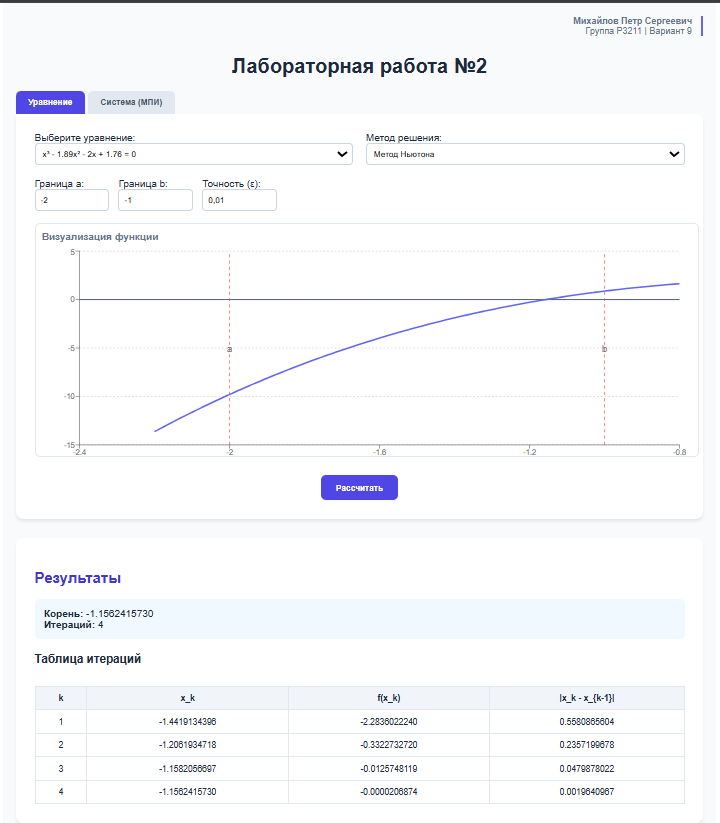
\includegraphics[width=0.85\textwidth]{screenshot_1.png}
    \caption{Результат работы программы: нелинейное уравнение успешно решено}
    \label{fig:res_eq_success}
\end{figure}

\subsection{Решение системы нелинейных уравнений}
На рисунке \ref{fig:res_sys_success} представлен результат решения системы уравнений с визуализацией пересечения графиков (линий уровня), что позволяет наглядно оценить корректность выбранного начального приближения.

\begin{figure}[H]
    \centering
    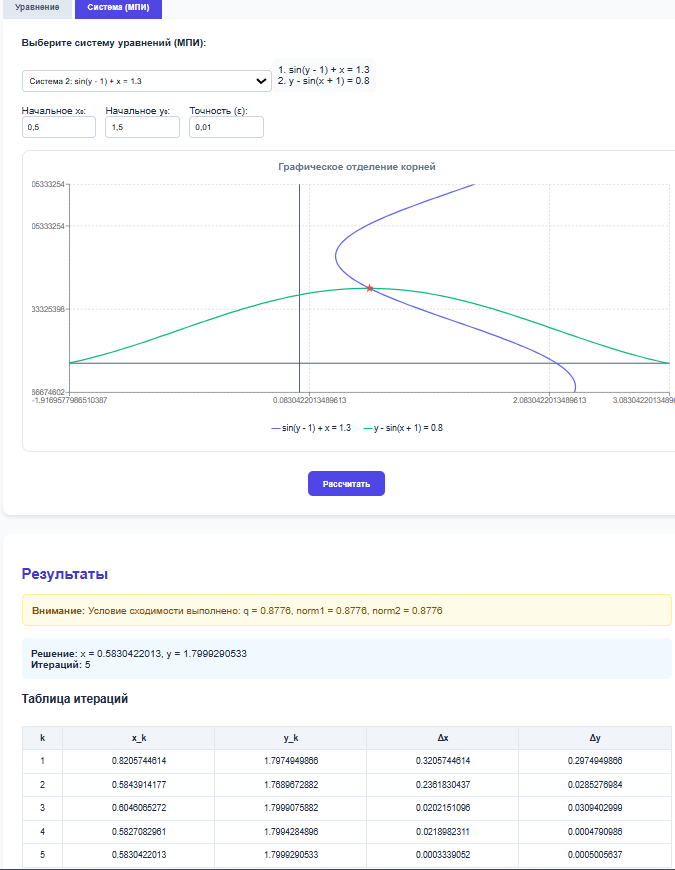
\includegraphics[width=0.85\textwidth]{screenshot_2.png}
    \caption{Результат работы программы: система уравнений успешно решена}
    \label{fig:res_sys_success}
\end{figure}

\subsection{Обработка некорректных входных данных}
Программа выполняет валидацию введенных данных и информирует пользователя, если на заданном интервале нет корней (знаки функции на концах отрезка совпадают) или если метод расходится.

\begin{figure}[H]
    \centering
    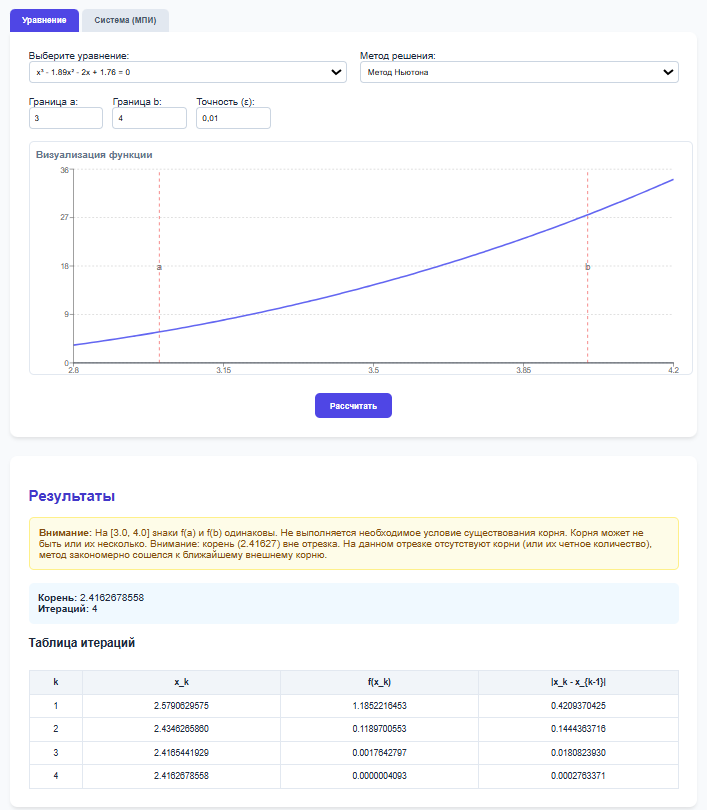
\includegraphics[width=0.85\textwidth]{screenshot_3.png}
    \caption{Реакция программы на отсутствие корня на выбранном интервале}
    \label{fig:res_error}
\end{figure}

% ===========================================================================
% 10. Выводы
% ===========================================================================
\newpage
\section{Выводы}
В ходе выполнения лабораторной работы были изучены и практически применены численные методы решения нелинейных уравнений и систем нелинейных уравнений. Выполнена программная реализация методов половинного деления, секущих, простой итерации, хорд и метода Ньютона.

На основе полученных аналитических и программных результатов можно сделать следующие выводы:
\begin{itemize}
    \item \textbf{Необходимость локализации корней:} Ключевым и обязательным этапом перед применением любого численного метода является локализация (отделение) корней. Использование графического метода позволяет визуально определить количество корней и сузить интервалы поиска, что критически важно для обеспечения сходимости итерационных процессов.
    \item \textbf{Сходимость и скорость методов:} Различные численные методы демонстрируют разную скорость сходимости и имеют разные требования к исходным данным. Метод половинного деления обладает гарантированной сходимостью для непрерывных функций, меняющих знак на интервале, но сходится относительно медленно. Метод Ньютона обладает высокой (квадратичной) скоростью сходимости, однако требует вычисления производной и весьма чувствителен к выбору начального приближения.
    \item \textbf{Особенности метода простой итерации:} Данный метод удобен для программной реализации, так как требует лишь вычисления значения самой функции на каждом шаге. Однако для его успешного применения необходимо предварительно провести математический анализ функции и подобрать параметр $\lambda$ так, чтобы выполнялось достаточное условие сходимости ($\max |\varphi'(x)| < 1$ на интервале).
    \item \textbf{Решение систем нелинейных уравнений:} Переход от одиночных уравнений к системам существенно усложняет задачу. Численное решение систем (в частности, методом Ньютона) требует на каждом итерационном шаге вычисления элементов матрицы Якоби и решения соответствующей системы линейных алгебраических уравнений (СЛАУ).
\end{itemize}

Разработанное программное обеспечение успешно решает поставленные задачи, обеспечивает наглядную графическую визуализацию процессов и контролирует корректность входных данных. Совпадение результатов ручных (табличных) расчетов с результатами работы программы подтверждает правильность реализованных численных алгоритмов.

\end{document}